\begin{figure}
\centering
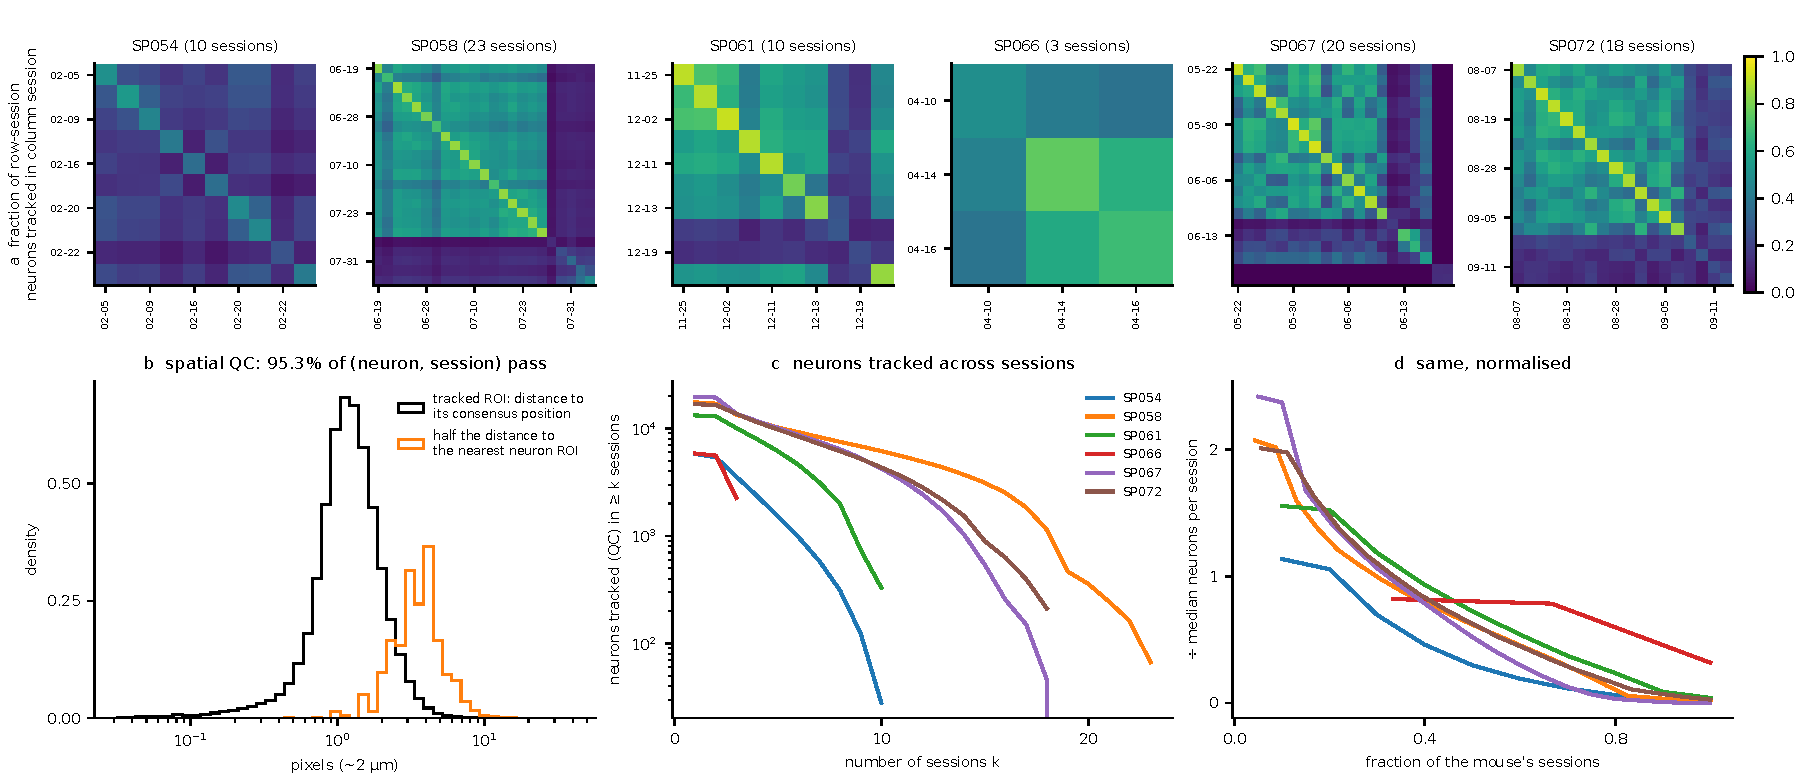
\includegraphics[width=\textwidth]{tracking_qc.pdf}
\caption{\textbf{Tracking QC of ROICaT neuron identities.} The ROICaT mirror gives only cluster IDs, so tracking was checked from ROI pixel positions: every pair of (session, FOV) sharing $\geq$20 tracked neurons was registered with a robust affine transform; a neuron's deviation in a session is the median residual over its pairs, and the match passes when it is smaller than half the distance to the nearest other neuron ROI (it cannot be a swap with that neighbour).
\textbf{a}~Fraction of each session's isocortex neurons tracked (QC passed) in every other session, per mouse. Low rows/columns: sessions with different coverage; SP058, SP067 and SP072 end with a block of sessions sharing few neurons with the earlier ones.
\textbf{b}~Distribution of deviations (black) vs.\ half the nearest-neighbour distance (orange); pixels are $\sim$2.5$\times$1.7~\textmu m. 95\% of (neuron, session) entries pass.
\textbf{c}~Number of neurons tracked in at least $k$ sessions per mouse. \textbf{d}~Same, normalised by the mouse's number of sessions and median number of neurons per session.}
\label{fig:tracking_qc}
\end{figure}
